\documentclass[notes,11pt, aspectratio=169]{beamer}

\usepackage{pgfpages}
\setbeameroption{hide notes} % Only slide

\usepackage{array}
\usepackage{tikz}
\usepackage{verbatim}
\setbeamertemplate{note page}{\pagecolor{gray!5}\insertnote}
\usetikzlibrary{positioning}
\usetikzlibrary{snakes}
\usetikzlibrary{calc}
\usetikzlibrary{arrows}
\usetikzlibrary{decorations.markings}
\usetikzlibrary{shapes.misc}
\usetikzlibrary{matrix,shapes,arrows,fit,tikzmark}
\usepackage{amsmath}
\usepackage{mathpazo}
\usepackage{hyperref}
\usepackage{lipsum}
\usepackage{multimedia}
\usepackage{graphicx}
\usepackage{multirow}
\usepackage{dcolumn}
\usepackage{bbm}
\newcolumntype{d}[0]{D{.}{.}{5}}

\usepackage{changepage}
\usepackage{appendixnumberbeamer}

\usepackage[space]{grffile}
\usepackage{booktabs}

% Colors
\definecolor{blue}{RGB}{0,114,178}
\definecolor{red}{RGB}{213,94,0}
\definecolor{yellow}{RGB}{240,228,66}
\definecolor{green}{RGB}{0,158,115}
\definecolor{solutionbg}{RGB}{240,248,240}
\definecolor{solutionframe}{RGB}{0,158,115}

% Solution box environment for worked answers
\usepackage{tcolorbox}
\newtcolorbox{solutionbox}[1][]{
  enhanced,
  colback=solutionbg,
  colframe=solutionframe,
  boxrule=0pt,
  leftrule=3pt,
  arc=0pt,
  left=8pt,
  right=8pt,
  top=6pt,
  bottom=6pt,
  fonttitle=\bfseries,
  title={#1},
  attach boxed title to top left={yshift=-2mm, xshift=5mm},
  boxed title style={colback=solutionframe, colframe=solutionframe, size=small, arc=2pt}
}

\hypersetup{
  colorlinks=false,
  linkbordercolor = {white},
  linkcolor = {blue}
}

\definecolor{MyBackground}{RGB}{255,253,218}

\newenvironment{transitionframe}{
  \setbeamercolor{background canvas}{bg=white}
  \begin{frame}}{
    \end{frame}
}

\setbeamercolor{frametitle}{fg=blue}
\setbeamercolor{title}{fg=black}
\setbeamertemplate{footline}[frame number]
\setbeamertemplate{navigation symbols}{}
\setbeamertemplate{itemize items}{-}
\setbeamercolor{itemize item}{fg=blue}
\setbeamercolor{itemize subitem}{fg=blue}
\setbeamercolor{enumerate item}{fg=blue}
\setbeamercolor{enumerate subitem}{fg=blue}
\setbeamercolor{button}{bg=MyBackground,fg=blue,}

\setbeamercolor{section in toc}{fg=blue}
\setbeamercolor{subsection in toc}{fg=red}
\setbeamersize{text margin left=1em,text margin right=1em}

\newenvironment{wideitemize}{\itemize\addtolength{\itemsep}{10pt}}{\enditemize}
\newenvironment{wideenumerate}{\enumerate\addtolength{\itemsep}{10pt}}{\endenumerate}

\title[]{\textcolor{blue}{ECN 594: Oligopoly Competition}}
\author[PGP]{}
\institute[FRBNY]{\small{\begin{tabular}{c c c}
Nicholas Vreugdenhil \\
\end{tabular}}}
\date{\today}

\begin{document}

% Title Slide
\begin{frame}
\maketitle
  \centering
\end{frame}

\begin{frame}{Welcome to Part 2}
	\begin{wideitemize}
		\item Demand estimation and pricing
		\item \textbf{Models of competition and industry structure}
		\begin{wideitemize}
			\vspace{5pt}
			\item Oligopoly models (Cournot, Bertrand, Hotelling)
			\item Entry and entry deterrence
			\item Mergers
			\item Vertical relationships
			\item Collusion
		\end{wideitemize}
		\item \textbf{HW2 released:} Merger simulation module
	\end{wideitemize}
\end{frame}

\begin{frame}{Plan}
  \begin{wideenumerate}
    \item \textbf{Cournot competition (refresher in IO notation)}
    \item Bertrand competition (refresher)
    \item Cournot vs Bertrand: when does each apply?
    \item Product differentiation: why it matters
    \item Hotelling model
    \item Connection to demand estimation
  \end{wideenumerate}
\end{frame}

%%%%%%%%%%%%%%%%%%%%%%%%%%%%%%%%%%%%%%%%%%%%%%%%%%%%%%%%%%%%%
% COURNOT AND BERTRAND
%%%%%%%%%%%%%%%%%%%%%%%%%%%%%%%%%%%%%%%%%%%%%%%%%%%%%%%%%%%%%

\begin{frame}{From ECN 532: Oligopoly models}
	\begin{wideitemize}
		\item You covered Cournot and Bertrand in Hector's class
		\item Today: quick refresher in IO notation
		\item \textbf{New focus:} Market power measurement
		\begin{wideitemize}
			\vspace{5pt}
			\item Connecting oligopoly models to Lerner index
			\item When does each model apply?
		\end{wideitemize}
	\end{wideitemize}
\end{frame}

\begin{frame}{Cournot competition: setup}
	\begin{wideitemize}
		\item $n$ firms producing homogeneous goods
		\item Firms choose \textbf{quantities} simultaneously
		\item Inverse demand: $P = P(Q)$ where $Q = \sum_{i=1}^n q_i$
		\item Constant marginal cost: $c$
		\item Firm $i$ profit: $\pi_i = P(Q) \cdot q_i - c \cdot q_i$
	\end{wideitemize}
\end{frame}

\begin{frame}{Cournot: first-order conditions}
	\begin{wideitemize}
		\item Firm $i$ maximizes profit taking $q_{-i}$ as given:
		\begin{align*}
			\frac{\partial \pi_i}{\partial q_i} = P(Q) + P'(Q) q_i - c = 0
		\end{align*}
		\item Rearranging:
		\begin{align*}
			P(Q) - c = -P'(Q) q_i
		\end{align*}
		\item Divide by $P$:
		\begin{align*}
			\frac{P - c}{P} = \frac{-P'(Q) q_i}{P} = \frac{-P'(Q) Q}{P} \cdot \frac{q_i}{Q} = \frac{s_i}{|\varepsilon|}
		\end{align*}
		\item where $s_i = q_i/Q$ is firm $i$'s market share
	\end{wideitemize}
\end{frame}

\begin{frame}{Cournot: Lerner index}
	\begin{wideitemize}
		\item \textbf{Key result:} In Cournot equilibrium,
		\begin{align*}
			L_i = \frac{P - MC}{P} = \frac{s_i}{|\varepsilon|}
		\end{align*}
		\item \textbf{Interpretation:}
		\begin{wideitemize}
			\vspace{5pt}
			\item Markup depends on market share
			\item Larger firms have more market power
			\item More elastic demand $\rightarrow$ lower markup
		\end{wideitemize}
		\item This connects to demand estimation from Part 1!
	\end{wideitemize}
\end{frame}

\begin{frame}{Worked example: Cournot with market power}
	\begin{wideitemize}
		\item \textbf{Question:} Inverse demand is $P = 100 - Q$. Two symmetric firms with $MC = 10$.
		\item (a) Find equilibrium quantities and price.
		\item (b) Calculate the Lerner index for each firm.
		\item (c) Verify using the $L = s/|\varepsilon|$ formula.
	\end{wideitemize}
	\vspace{10pt}
	\centering
	\textit{Take 5 minutes.}
\end{frame}

\begin{frame}{Worked example: Cournot (solution)}
	\begin{solutionbox}[Solution]
		\begin{wideitemize}
			\item \textbf{(a)} FOC: $100 - 2q_i - q_j - 10 = 0$
			\item Symmetric: $q_1 = q_2 = q^*$, so $100 - 3q^* = 10 \Rightarrow q^* = 30$
			\item $Q = 60$, $P = 100 - 60 = 40$
			\item \textbf{(b)} $L = \frac{40 - 10}{40} = \frac{3}{4} = 0.75$
			\item \textbf{(c)} Market share: $s_i = 30/60 = 0.5$
			\item Elasticity: $\varepsilon = \frac{dQ}{dP} \cdot \frac{P}{Q} = (-1) \cdot \frac{40}{60} = -\frac{2}{3}$
			\item Check: $L = \frac{s_i}{|\varepsilon|} = \frac{0.5}{2/3} = 0.75$ $\checkmark$
		\end{wideitemize}
	\end{solutionbox}
\end{frame}

\begin{frame}{Cournot with $n$ symmetric firms}
	\begin{wideitemize}
		\item General result for linear demand $P = a - bQ$:
		\item Symmetric equilibrium: $q^* = \frac{a - c}{b(n+1)}$
		\item Total quantity: $Q^* = \frac{n(a-c)}{b(n+1)}$
		\item Price: $P^* = \frac{a + nc}{n+1}$
		\item Lerner index: $L = \frac{1}{n|\varepsilon|}$ (symmetric case where $s_i = 1/n$)
		\item \textbf{Key insight:} As $n \to \infty$, $P \to MC$ (perfect competition)
	\end{wideitemize}
\end{frame}

\begin{frame}{Practice: Cournot comparative statics}
	\begin{wideitemize}
		\item \textbf{True, False, or NEI:}
		\item (a) In Cournot equilibrium, a firm with a larger market share has a higher markup.
		\item (b) Adding a third firm to a Cournot duopoly always reduces industry profits.
		\item (c) In Cournot, all firms must have the same marginal cost.
	\end{wideitemize}
	\vspace{10pt}
	\centering
	\textit{Take 2 minutes.}
\end{frame}

\begin{frame}{Practice: Cournot comparative statics (solution)}
	\begin{solutionbox}[Answers]
		\begin{wideitemize}
			\item \textbf{(a) TRUE.} From $L_i = s_i/|\varepsilon|$, larger $s_i$ means higher $L_i$.
			\item \textbf{(b) TRUE.} More firms $\Rightarrow$ lower price $\Rightarrow$ lower industry profit. Each firm's profit falls, and total profit falls because $P$ is closer to $MC$.
			\item \textbf{(c) FALSE.} Asymmetric costs work fine. Low-cost firms have higher $q_i$ and $s_i$, hence higher margins.
		\end{wideitemize}
	\end{solutionbox}
\end{frame}

\begin{frame}{Plan}
  \begin{wideenumerate}
    \item Cournot competition (refresher in IO notation)
    \item \textbf{Bertrand competition (refresher)}
    \item Cournot vs Bertrand: when does each apply?
    \item Product differentiation: why it matters
    \item Hotelling model
    \item Connection to demand estimation
  \end{wideenumerate}
\end{frame}

\begin{frame}{Bertrand competition: setup}
	\begin{wideitemize}
		\item $n$ firms producing \textbf{homogeneous} goods
		\item Firms choose \textbf{prices} simultaneously
		\item Consumers buy from lowest-price firm
		\item If tie: split demand equally
		\item Constant marginal cost: $c$
	\end{wideitemize}
\end{frame}

\begin{frame}{Bertrand: the paradox}
	\begin{wideitemize}
		\item \textbf{Nash equilibrium:} $p_1 = p_2 = c$ (marginal cost pricing!)
		\item \textbf{Why?}
		\begin{wideitemize}
			\vspace{5pt}
			\item If $p_i > p_j > c$: firm $i$ can undercut and capture entire market
			\item Undercutting continues until $p = c$
		\end{wideitemize}
		\item \textbf{The ``paradox'':}
		\begin{wideitemize}
			\vspace{5pt}
			\item Only 2 firms, but competitive outcome!
			\item Zero profits with just 2 competitors
			\item Seems unrealistic for most markets
		\end{wideitemize}
	\end{wideitemize}
\end{frame}

\begin{frame}{Plan}
  \begin{wideenumerate}
    \item Cournot competition (refresher in IO notation)
    \item Bertrand competition (refresher)
    \item \textbf{Cournot vs Bertrand: when does each apply?}
    \item Product differentiation: why it matters
    \item Hotelling model
    \item Connection to demand estimation
  \end{wideenumerate}
\end{frame}

\begin{frame}{Cournot vs Bertrand: summary}
	\begin{center}
		\begin{tabular}{|l|c|c|}
			\hline
			& \textbf{Cournot} & \textbf{Bertrand} \\
			\hline
			Strategic variable & Quantities & Prices \\
			\hline
			Equilibrium price & $P > MC$ & $P = MC$ \\
			\hline
			Profits & Positive & Zero \\
			\hline
			Lerner index & $L = s/|\varepsilon|$ & $L = 0$ \\
			\hline
		\end{tabular}
	\end{center}
	\vspace{10pt}
	\begin{wideitemize}
		\item Which model is ``right''?
		\item Answer: depends on the industry!
	\end{wideitemize}
\end{frame}

\begin{frame}{Escaping the Bertrand paradox}
	\begin{wideenumerate}
		\item \textbf{Capacity constraints} (Kreps-Scheinkman)
		\begin{wideitemize}
			\vspace{3pt}
			\item Can't serve entire market at low price
			\item Leads to Cournot outcome
		\end{wideitemize}
		\item \textbf{Product differentiation} (today's main topic!)
		\begin{wideitemize}
			\vspace{3pt}
			\item Consumers have preferences
			\item Not all switch to lowest price
		\end{wideitemize}
		\item \textbf{Repeated interaction} (collusion, covered later)
		\begin{wideitemize}
			\vspace{3pt}
			\item Firms can sustain $P > MC$ through punishment strategies
		\end{wideitemize}
	\end{wideenumerate}
\end{frame}

\begin{frame}{When does each model apply?}
	\begin{wideitemize}
		\item \textbf{Cournot applies when:}
		\begin{wideitemize}
			\vspace{5pt}
			\item Capacity constraints matter
			\item Firms commit to production before selling
			\item Quantities are hard to adjust quickly
		\end{wideitemize}
		\item Examples: manufacturing, airlines (seat capacity)
		\item \textbf{Bertrand applies when:}
		\begin{wideitemize}
			\vspace{5pt}
			\item Prices adjust quickly
			\item No capacity constraints
			\item Homogeneous products
		\end{wideitemize}
		\item Examples: online retail, commodities
	\end{wideitemize}
\end{frame}

\begin{frame}{Industry examples: which model?}
	\begin{center}
	\begin{tabular}{|l|c|l|}
		\hline
		\textbf{Industry} & \textbf{Model} & \textbf{Why?} \\
		\hline
		Airlines & Cournot & Capacity (planes, gates) committed \\
		\hline
		Cement & Cournot & Production committed; transport costs \\
		\hline
		Gasoline stations & Bertrand & Prices adjust daily; commodity \\
		\hline
		Online retail & Bertrand & Instant price changes; no capacity \\
		\hline
		Smartphones & Differentiated & Product differentiation dominates \\
		\hline
	\end{tabular}
	\end{center}
	\vspace{5pt}
	\begin{wideitemize}
		\item In practice: most markets have differentiated products!
	\end{wideitemize}
\end{frame}

\begin{frame}{Practice: Cournot vs Bertrand}
	\begin{wideitemize}
		\item \textbf{Question:} Two firms have $MC = 20$. Market demand is $P = 100 - Q$.
		\item (a) Find equilibrium price under Cournot.
		\item (b) Find equilibrium price under Bertrand.
		\item (c) Which model yields higher consumer surplus? Why?
	\end{wideitemize}
	\vspace{10pt}
	\centering
	\textit{Take 3 minutes.}
\end{frame}

\begin{frame}{Practice: Cournot vs Bertrand (solution)}
	\begin{solutionbox}[Solution]
		\begin{wideitemize}
			\item \textbf{(a) Cournot:} Using $P^* = \frac{a + nc}{n+1} = \frac{100 + 2(20)}{3} = 46.67$
			\item Or: $q^* = \frac{100-20}{3} = 26.67$, $Q = 53.33$, $P = 46.67$
			\item \textbf{(b) Bertrand:} $P = MC = 20$
			\item \textbf{(c)} Bertrand has higher CS:
			\begin{wideitemize}
				\vspace{5pt}
				\item Bertrand: $CS = \frac{1}{2}(100-20)(80) = 3200$
				\item Cournot: $CS = \frac{1}{2}(100-46.67)(53.33) \approx 1422$
			\end{wideitemize}
			\item Lower price $\Rightarrow$ higher quantity $\Rightarrow$ higher CS
		\end{wideitemize}
	\end{solutionbox}
\end{frame}

\begin{frame}{Kreps-Scheinkman (1983): resolving the puzzle}
	\begin{wideitemize}
		\item Two-stage game:
		\begin{wideenumerate}
			\vspace{5pt}
			\item Stage 1: Firms choose capacities (quantities)
			\item Stage 2: Firms compete in prices
		\end{wideenumerate}
		\item \textbf{Result:} Equilibrium outcome = Cournot!
		\item \textbf{Intuition:}
		\begin{wideitemize}
			\vspace{5pt}
			\item Capacity choice commits firms
			\item Price competition is constrained by capacity
			\item Undercutting is limited by what you can produce
		\end{wideitemize}
		\item Key insight: commitment matters
	\end{wideitemize}
\end{frame}

%%%%%%%%%%%%%%%%%%%%%%%%%%%%%%%%%%%%%%%%%%%%%%%%%%%%%%%%%%%%%
% HOTELLING MODEL
%%%%%%%%%%%%%%%%%%%%%%%%%%%%%%%%%%%%%%%%%%%%%%%%%%%%%%%%%%%%%

\begin{frame}{Plan}
  \begin{wideenumerate}
    \item Cournot competition (refresher in IO notation)
    \item Bertrand competition (refresher)
    \item Cournot vs Bertrand: when does each apply?
    \item \textbf{Product differentiation: why it matters}
    \item Hotelling model
    \item Connection to demand estimation
  \end{wideenumerate}
\end{frame}

\begin{frame}{Why differentiation matters}
	\begin{wideitemize}
		\item Bertrand paradox: $P = MC$ with homogeneous products
		\item \textbf{Solution:} Product differentiation!
		\item If products are different, consumers don't all buy from lowest-price firm
		\item Firms have some pricing power
		\item This is exactly what we modeled in Part 1 (logit demand)
		\item Now: a classic spatial model of differentiation
	\end{wideitemize}
\end{frame}

\begin{frame}{Plan}
  \begin{wideenumerate}
    \item Cournot competition (refresher in IO notation)
    \item Bertrand competition (refresher)
    \item Cournot vs Bertrand: when does each apply?
    \item Product differentiation: why it matters
    \item \textbf{Hotelling model}
    \item Connection to demand estimation
  \end{wideenumerate}
\end{frame}

\begin{frame}{Hotelling model: setup}
	\begin{wideitemize}
		\item Consumers uniformly distributed on $[0, 1]$ (``Main Street'')
		\item Two firms located at positions $a$ and $b$ on $[0, 1]$
		\item Consumer at location $x$ has utility:
		\begin{align*}
			u_j = v - p_j - t|x - \ell_j|
		\end{align*}
		\item $v$: base value of product
		\item $p_j$: price of firm $j$
		\item $t$: transport cost per unit distance
		\item $|x - \ell_j|$: distance to firm $j$
	\end{wideitemize}
\end{frame}

\begin{frame}{Hotelling: graphical intuition}
	\begin{center}
		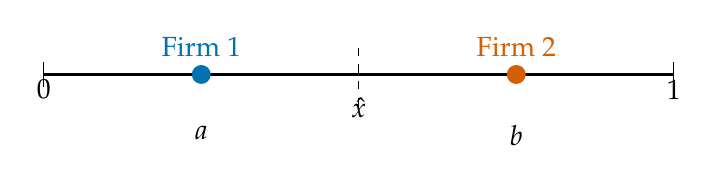
\begin{tikzpicture}[scale=8]
			% Main line
			\draw[thick] (0,0) -- (1,0);
			\draw (0,-0.02) -- (0,0.02) node[below=3pt] {$0$};
			\draw (1,-0.02) -- (1,0.02) node[below=3pt] {$1$};

			% Firms
			\fill[blue] (0.25,0) circle (0.015) node[above=3pt] {Firm 1};
			\fill[red] (0.75,0) circle (0.015) node[above=3pt] {Firm 2};

			% Indifferent consumer
			\draw[dashed] (0.5,-0.05) -- (0.5,0.05);
			\node[below=5pt] at (0.5,0) {$\hat{x}$};

			% Labels
			\node[below=15pt] at (0.25,0) {$a$};
			\node[below=15pt] at (0.75,0) {$b$};
		\end{tikzpicture}
	\end{center}
	\begin{wideitemize}
		\item Consumers to the left of $\hat{x}$ buy from Firm 1
		\item Consumers to the right of $\hat{x}$ buy from Firm 2
		\item $\hat{x}$ is the ``indifferent consumer''
	\end{wideitemize}
\end{frame}

\begin{frame}{Finding the indifferent consumer}
	\begin{wideitemize}
		\item Consumer at $\hat{x}$ is indifferent between firms:
		\begin{align*}
			v - p_1 - t|\hat{x} - a| = v - p_2 - t|b - \hat{x}|
		\end{align*}
		\item With $a = 0$ and $b = 1$ (firms at endpoints):
		\begin{align*}
			v - p_1 - t\hat{x} &= v - p_2 - t(1 - \hat{x}) \\
			p_2 - p_1 &= t(1 - 2\hat{x}) \\
			\hat{x} &= \frac{1}{2} + \frac{p_2 - p_1}{2t}
		\end{align*}
		\item Demand for firm 1: $D_1 = \hat{x}$
		\item Demand for firm 2: $D_2 = 1 - \hat{x}$
	\end{wideitemize}
\end{frame}

\begin{frame}{Hotelling: equilibrium prices}
	\begin{wideitemize}
		\item Firm 1 maximizes: $\pi_1 = (p_1 - c) \cdot \hat{x}(p_1, p_2)$
		\item FOC: $\frac{\partial \pi_1}{\partial p_1} = \hat{x} + (p_1 - c) \frac{\partial \hat{x}}{\partial p_1} = 0$
		\item With $\frac{\partial \hat{x}}{\partial p_1} = -\frac{1}{2t}$:
		\begin{align*}
			\frac{1}{2} + \frac{p_2 - p_1}{2t} - \frac{p_1 - c}{2t} = 0
		\end{align*}
		\item Symmetric equilibrium ($p_1 = p_2 = p^*$):
		\begin{align*}
			p^* = c + t
		\end{align*}
		\item \textbf{Markup = transport cost!}
	\end{wideitemize}
\end{frame}

\begin{frame}{Hotelling: interpretation}
	\begin{wideitemize}
		\item $p^* = c + t$: Firms charge above marginal cost
		\item \textbf{Transport cost $t$ measures differentiation}
		\begin{wideitemize}
			\vspace{5pt}
			\item High $t$: products very different $\rightarrow$ high markup
			\item Low $t$: products similar $\rightarrow$ low markup
			\item $t \to 0$: products identical $\rightarrow$ Bertrand ($p \to c$)
		\end{wideitemize}
		\item \textbf{No Bertrand paradox:} Differentiation creates pricing power
		\item Each firm gets half the market: $D_1 = D_2 = 1/2$
		\item Profit: $\pi = (p^* - c) \cdot \frac{1}{2} = \frac{t}{2}$
	\end{wideitemize}
\end{frame}

\begin{frame}{Worked example: Hotelling}
	\begin{wideitemize}
		\item \textbf{Question:} Two ice cream vendors on a beach of length 1 mile. Transport cost $t = 2$ dollars per mile. Marginal cost $c = 1$.
		\item (a) Find the equilibrium price.
		\item (b) If firm 1 raises price to $p_1 = 4$, what is its market share?
		\item (c) Calculate firm 1's demand elasticity at the equilibrium.
	\end{wideitemize}
	\vspace{10pt}
	\centering
	\textit{Take 4 minutes.}
\end{frame}

\begin{frame}{Worked example: Hotelling (solution)}
	\begin{solutionbox}[Solution]
		\begin{wideitemize}
			\item \textbf{(a)} $p^* = c + t = 1 + 2 = 3$
			\item \textbf{(b)} At $p_1 = 4$, $p_2 = 3$:
			\begin{align*}
				\hat{x} = \frac{1}{2} + \frac{3 - 4}{2(2)} = \frac{1}{2} - \frac{1}{4} = \frac{1}{4}
			\end{align*}
			\item Firm 1's market share falls to 25\%
			\item \textbf{(c)} At equilibrium: $D_1 = 1/2$, $\frac{\partial D_1}{\partial p_1} = -\frac{1}{2t} = -\frac{1}{4}$
			\begin{align*}
				\varepsilon_1 = \frac{\partial D_1}{\partial p_1} \cdot \frac{p_1}{D_1} = -\frac{1}{4} \cdot \frac{3}{1/2} = -1.5
			\end{align*}
		\end{wideitemize}
	\end{solutionbox}
\end{frame}

\begin{frame}{Hotelling: why transport cost matters}
	\begin{wideitemize}
		\item \textbf{High $t$:} Strong differentiation
		\begin{wideitemize}
			\vspace{5pt}
			\item Consumers have strong location preferences
			\item Firm can raise price without losing many customers
			\item Example: specialty restaurants vs fast food
		\end{wideitemize}
		\item \textbf{Low $t$:} Weak differentiation
		\begin{wideitemize}
			\vspace{5pt}
			\item Consumers nearly indifferent across locations
			\item Small price cut steals many customers
			\item Approaches Bertrand as $t \to 0$
		\end{wideitemize}
		\item In demand estimation: $1/\alpha$ plays similar role to $t$
	\end{wideitemize}
\end{frame}

\begin{frame}{Practice: T/F on Hotelling}
	\begin{wideitemize}
		\item \textbf{True, False, or NEI:}
		\item (a) In Hotelling equilibrium, firms always split the market equally.
		\item (b) A monopolist in Hotelling should locate at the center of the line.
		\item (c) Higher transport costs benefit consumers because products are more differentiated.
	\end{wideitemize}
	\vspace{10pt}
	\centering
	\textit{Take 2 minutes.}
\end{frame}

\begin{frame}{Practice: T/F on Hotelling (solution)}
	\begin{solutionbox}[Answers]
		\begin{wideitemize}
			\item \textbf{(a) TRUE} (with caveat). If firms are at endpoints and have same costs, yes. With asymmetric locations or costs, shares differ.
			\item \textbf{(b) TRUE.} Monopolist minimizes total transport costs by locating at center. This maximizes consumer value and thus WTP.
			\item \textbf{(c) FALSE.} Higher $t$ means higher prices ($p^* = c + t$) and higher transport costs. Both hurt consumers.
		\end{wideitemize}
	\end{solutionbox}
\end{frame}

\begin{frame}{Welfare in Hotelling}
	\begin{wideitemize}
		\item \textbf{Total welfare} = Consumer surplus + Profits
		\item Transport costs are deadweight loss
		\item \textbf{Socially optimal locations:} $a = 1/4$, $b = 3/4$
		\begin{wideitemize}
			\vspace{5pt}
			\item Minimizes total transport costs
		\end{wideitemize}
		\item \textbf{Equilibrium locations:} Both firms at $1/2$ (minimum differentiation)
		\begin{wideitemize}
			\vspace{5pt}
			\item Firms want to capture more customers
			\item But this increases total transport costs
		\end{wideitemize}
		\item ``Principle of minimum differentiation'' (but fragile)
	\end{wideitemize}
\end{frame}

\begin{frame}{Plan}
  \begin{wideenumerate}
    \item Cournot competition (refresher in IO notation)
    \item Bertrand competition (refresher)
    \item Cournot vs Bertrand: when does each apply?
    \item Product differentiation: why it matters
    \item Hotelling model
    \item \textbf{Connection to demand estimation}
  \end{wideenumerate}
\end{frame}

\begin{frame}{Connection to demand estimation}
	\begin{wideitemize}
		\item Hotelling is a specific \textbf{differentiated Bertrand} model
		\item Location $\leftrightarrow$ product characteristics
		\item Transport cost $\leftrightarrow$ preference heterogeneity
		\item \textbf{Logit demand} generalizes this idea:
		\begin{wideitemize}
			\vspace{5pt}
			\item Products differ in characteristics space
			\item Consumers have heterogeneous preferences
			\item Price competition with differentiated products
		\end{wideitemize}
		\item Next lectures: how to use demand estimates for merger simulation
	\end{wideitemize}
\end{frame}

\begin{frame}{From Hotelling to logit: the connection}
	\begin{center}
	\begin{tabular}{|l|l|}
		\hline
		\textbf{Hotelling} & \textbf{Logit} \\
		\hline
		Location on line & Product characteristics \\
		\hline
		Transport cost $t$ & Sensitivity $1/|\alpha|$ \\
		\hline
		Consumer position & Consumer preferences \\
		\hline
		Linear utility & Logit choice probabilities \\
		\hline
		2 products & $J$ products \\
		\hline
	\end{tabular}
	\end{center}
	\vspace{5pt}
	\begin{wideitemize}
		\item Logit demand lets us do empirical Hotelling-style analysis
		\item Estimate $\alpha$ from data $\rightarrow$ calibrate ``differentiation''
	\end{wideitemize}
\end{frame}

\begin{frame}{Oligopoly models: summary}
	\begin{wideitemize}
		\item \textbf{Homogeneous products:}
		\begin{wideitemize}
			\vspace{5pt}
			\item Cournot (quantity): $L = s_i/|\varepsilon|$
			\item Bertrand (price): $P = MC$
		\end{wideitemize}
		\item \textbf{Differentiated products:}
		\begin{wideitemize}
			\vspace{5pt}
			\item Hotelling/Differentiated Bertrand: $P > MC$
			\item Markup depends on differentiation (transport cost)
		\end{wideitemize}
		\item \textbf{Empirical approach:}
		\begin{wideitemize}
			\vspace{5pt}
			\item Estimate demand (logit)
			\item Assume pricing behavior (usually differentiated Bertrand)
			\item Back out marginal costs
		\end{wideitemize}
	\end{wideitemize}
\end{frame}

\begin{frame}{Preview: merger simulation}
	\begin{wideitemize}
		\item \textbf{Key question:} If two firms merge, what happens to prices?
		\item \textbf{Approach:}
		\begin{wideenumerate}
			\vspace{5pt}
			\item Estimate demand $\rightarrow$ get elasticities
			\item Assume Bertrand pricing $\rightarrow$ back out $MC$
			\item Change ownership structure
			\item Solve new Bertrand equilibrium
			\item Compare prices and welfare
		\end{wideenumerate}
		\item This is exactly what HW2 will do!
		\item Will cover in detail in Lecture 10
	\end{wideitemize}
\end{frame}

%%%%%%%%%%%%%%%%%%%%%%%%%%%%%%%%%%%%%%%%%%%%%%%%%%%%%%%%%%%%%
% KEY POINTS
%%%%%%%%%%%%%%%%%%%%%%%%%%%%%%%%%%%%%%%%%%%%%%%%%%%%%%%%%%%%%

\begin{frame}{Key Points}
	\vspace{11pt}
	\begin{wideenumerate}
		\item \textbf{Cournot:} Firms choose quantities; $L = s_i/|\varepsilon|$
		\item \textbf{Bertrand (homogeneous):} $P = MC$, zero profits
		\item \textbf{Bertrand paradox:} Only 2 firms but competitive outcome
		\item Cournot applies with capacity constraints; Bertrand with flexible prices
		\item \textbf{Product differentiation} creates pricing power
		\item \textbf{Hotelling:} $p^* = c + t$ (markup = transport cost)
		\item Higher $t$ (more differentiation) $\rightarrow$ higher markup
		\item Hotelling connects to logit demand from Part 1
	\end{wideenumerate}
\end{frame}

\begin{frame}{Next time}
	\begin{wideitemize}
		\item \textbf{Lecture 9:} Entry and Market Structure
		\begin{wideitemize}
			\vspace{5pt}
			\item Free entry condition
			\item Entry deterrence: limit pricing, excess capacity
			\item Strategic entry barriers
		\end{wideitemize}
	\end{wideitemize}
\end{frame}

\end{document}
